%!TEX root = ../main.tex
\chapter{Metodología de la investigación}\label{cap:metodologia}

\section{Área temática}

Este proyecto aborda la automatización de procesos financieros y administrativos. Concretamente, busca mejorar la gestión de la facturación de unidades financiadas en una compañía automotriz, para lo cual se integran sus sistemas internos con los de las entidades bancarias. La investigación se centra en mejorar las tareas operativas ligadas a la validación de líneas de crédito, con un objetivo triple: reducir los tiempos de ejecución, minimizar posibles errores y, fundamentalmente, fortalecer la trazabilidad de todo el proceso.

\section{Planteamiento del problema}

Actualmente, el proceso de actualización y validación de líneas de crédito para la facturación de unidades financiadas se realiza de forma manual, con saldos cargados a mano e intercambio de información mediante archivos por FTP o planillas de Excel, lo que genera demoras, errores y baja trazabilidad. Ante esta situación, se requiere investigar y desarrollar una solución que automatice el proceso, mejore el control operativo e integre de forma más eficiente los sistemas internos con entidades bancarias externas.

\section{Delimitación de la investigación}

La investigación se enfocará en el análisis, diseño e implementación de una solución para automatizar la validación de líneas de crédito y la facturación de unidades en una empresa automotriz. Se considerarán escenarios de operación en Chile y Perú, integrando entidades bancarias mediante API REST sobre una arquitectura modular que convive con el sistema legado existente. No se incluyen modificaciones a la operatoria interna de los bancos, migraciones completas de sistemas legados ni la implementación productiva en todos los mercados de la organización.

\section{Marco teórico}

Se revisarán los conceptos vinculados con automatización de procesos financieros, facturación de unidades financiadas, validación de líneas de crédito e integración de sistemas mediante FTP y API REST. Además, se estudiarán arquitecturas modulares, mecanismos de monitoreo, auditoría, trazabilidad y seguridad de la información aplicados a sistemas distribuidos. También se investigarán antecedentes y casos similares de integración entre sistemas empresariales y entidades bancarias.

\section{Diseño concreto de investigación}

La investigación tendrá un enfoque aplicado, con diseño orientado a la construcción de un prototipo funcional. Se analizará el proceso actual, se diseñará una solución con arquitectura modular y se implementará un modelo de integración mediante API REST. La propuesta será evaluada en entornos controlados mediante pruebas funcionales y de integración, comparando sus resultados con el proceso actual basado en tareas manuales y transferencia de archivos FTP.

\section{Indicadores}

Para evaluar la efectividad de la solución propuesta se utilizarán distintos indicadores que permitan medir el impacto de la automatización sobre el proceso de validación de líneas de crédito y facturación de unidades. Uno de los principales indicadores será el tiempo promedio requerido para procesar una validación de línea de crédito, ya que permitirá comparar la eficiencia del proceso actual con la obtenida mediante la solución desarrollada.

Asimismo, se analizará la cantidad de intervenciones manuales necesarias durante la ejecución de las operaciones, con el objetivo de determinar el grado de automatización alcanzado. También se considerará la cantidad de errores operativos detectados durante el procesamiento de las transacciones, así como la capacidad de identificar incidencias mediante los mecanismos de monitoreo y auditoría incorporados en la arquitectura propuesta.

Otro aspecto relevante será la trazabilidad de las operaciones, evaluando la disponibilidad de registros que permitan conocer el estado de cada transacción y reconstruir su historial en caso de ser necesario. Finalmente, se analizará la capacidad de integración con distintas entidades bancarias y la percepción de los usuarios respecto de la utilidad de la solución implementada y las mejoras obtenidas en comparación con el proceso actual.

\section{Técnicas de recolección de datos}

La recolección de datos se realizará mediante la revisión de documentación funcional y técnica de los sistemas involucrados, la observación directa del proceso actual de facturación y validación de líneas de crédito, y la realización de entrevistas con usuarios clave y referentes técnicos. Estas técnicas permitirán comprender el funcionamiento vigente, identificar puntos críticos y obtener información útil para el diseño de la solución propuesta.

Además, se ejecutarán pruebas funcionales, técnicas e integrales sobre el prototipo desarrollado, con el fin de observar su comportamiento en condiciones controladas y validar su correcto funcionamiento frente a escenarios representativos del proceso real. También se recopilarán resultados derivados de pruebas de integración con entidades bancarias o simulaciones de dichos servicios cuando no sea posible acceder a ambientes externos.

\section{Instrumentos de recolección de datos}

Para llevar adelante la recolección de datos se utilizarán distintos instrumentos acordes a cada técnica aplicada. Entre ellos se incluyen guías de entrevista, plantillas de observación, registros de pruebas, reportes de incidencias, logs de ejecución y documentación funcional y técnica de los sistemas existentes. Estos instrumentos permitirán organizar la información obtenida y asegurar su posterior análisis de manera ordenada.

Adicionalmente, se emplearán mecanismos de monitoreo, auditoría y registro de eventos incorporados en la solución propuesta, los cuales facilitarán el seguimiento de las operaciones, la detección de errores y la evaluación del comportamiento del sistema durante las instancias de prueba.

\section{Datos y procesamiento de datos}

Los datos utilizados en la investigación provendrán del relevamiento del proceso actual, de la documentación técnica y funcional disponible, de los resultados obtenidos en las pruebas del prototipo y de las métricas generadas por la solución implementada. En una primera instancia, estos datos se obtendrán en forma dispersa o en bruto, por lo que será necesario clasificarlos y organizarlos según su naturaleza y utilidad para el análisis.

Posteriormente, se llevará a cabo un proceso de depuración, consolidación y normalización de la información, con el objetivo de facilitar la comparación entre el esquema actual y la solución automatizada. Este procesamiento permitirá disponer de datos consistentes y ordenados para evaluar el desempeño del sistema y respaldar las conclusiones de la investigación.

Durante la elaboración del trabajo se utilizaron herramientas de inteligencia artificial: Perplexity AI para la búsqueda de antecedentes académicos y Claude, de Anthropic, para dar formato académico a contenidos elaborados por el autor, revisar la redacción y la coherencia entre capítulos y elaborar diagramas a partir de información provista por él. No se utilizó inteligencia artificial en el desarrollo del sistema. El alcance y las condiciones de uso se detallan en la Declaración sobre el uso de inteligencia artificial.

\section{Análisis de los datos}

El análisis de los datos se realizará a partir de los indicadores definidos previamente, comparando el comportamiento del proceso actual con el obtenido mediante la solución propuesta. Se buscará identificar variaciones en los tiempos de procesamiento, la cantidad de tareas manuales, la frecuencia de errores, el nivel de trazabilidad alcanzado y la capacidad de integración con las entidades bancarias involucradas.

A partir de esta comparación será posible evaluar el impacto real de la automatización en la operatoria del negocio, así como identificar eventuales mejoras, ajustes o necesidades adicionales para futuras iteraciones. De este modo, el análisis no solo permitirá validar la solución desarrollada, sino también determinar su viabilidad como base para una eventual ampliación a otros mercados.

\section{Síntesis y conclusiones}

Una vez analizados los resultados obtenidos, se elaborará una síntesis de los principales hallazgos de la investigación y se formularán las conclusiones finales. En esta instancia se determinará si la solución propuesta contribuye efectivamente a mejorar la eficiencia operativa, disminuir la intervención manual y fortalecer la trazabilidad del proceso de validación de líneas de crédito y facturación.

Asimismo, se considerarán las limitaciones observadas durante el desarrollo del trabajo y se podrán proponer recomendaciones para futuras mejoras, ajustes funcionales o extensiones de la solución a otros contextos operativos dentro de la organización o en otros países de la región.

\section{Detalle del proyecto}

\subsection{Alcance}

El alcance de la investigación comprende el análisis, diseño e implementación de una solución con arquitectura modular e integración mediante API REST para automatizar el proceso de validación de líneas de crédito y facturación de unidades en una empresa automotriz. La propuesta se validará en escenarios representativos de Chile y Perú, con foco en la mejora del proceso actual y en la evaluación de su funcionamiento en entornos controlados.

No se incluyen dentro del alcance modificaciones a la operatoria interna de las entidades bancarias, migraciones completas de los sistemas legados existentes, reemplazos totales de las plataformas corporativas actuales ni implementaciones productivas en todos los mercados donde opera la organización. Tampoco se contempla el desarrollo de infraestructura física adicional ni cambios estructurales fuera del proceso analizado.

\subsection{Tiempos}

El proyecto se desarrollará de manera progresiva a través de distintas etapas que reflejan tanto la elaboración de la investigación como la construcción de la solución propuesta. En una primera fase se prevé la revisión del estado del arte, el relevamiento del proceso actual y la definición del problema, objetivos e hipótesis. Luego se avanzará con el desarrollo del marco teórico, el diseño de la solución y la implementación de los componentes necesarios.

Posteriormente se llevarán a cabo pruebas funcionales, técnicas e integrales, junto con instancias de ajuste y validación. Finalmente, se realizará la redacción de conclusiones, la revisión general del documento y la preparación de la presentación final. El cronograma general del proyecto se presenta en la Figura~\ref{fig:1}, donde se detallan las fases de relevamiento, diseño, desarrollo, pruebas y puesta en producción de la solución, junto con la elaboración del documento. Las entregas de cada capítulo se indican como hitos.

\begin{figure}[H]
\centering
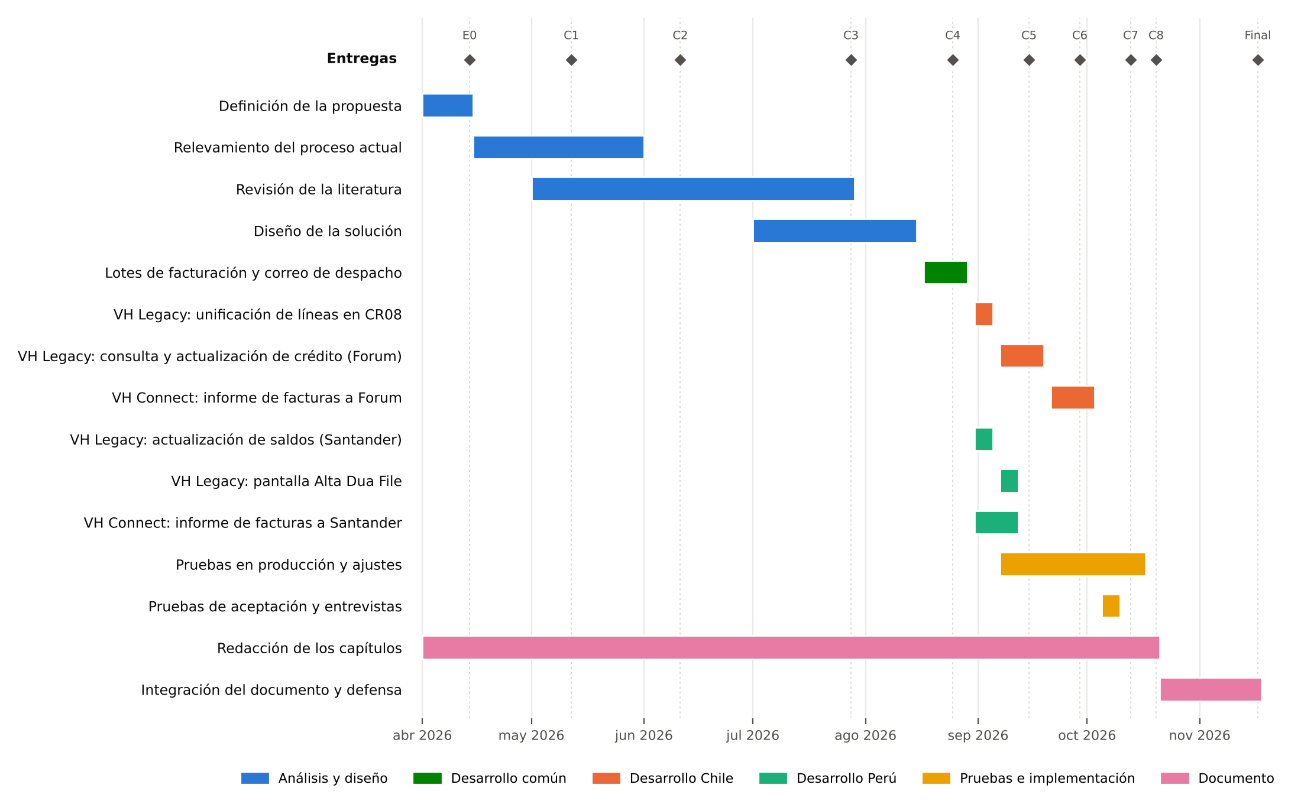
\includegraphics[width=1.00\textwidth]{figuras/image2}
\caption{Cronograma de actividades del proyecto}\label{fig:1}
\end{figure}

\subsection{Costos}

El proyecto no requiere una inversión económica significativa, ya que se desarrollará principalmente con recursos y herramientas disponibles dentro de la organización. Las actividades de análisis, diseño, desarrollo y prueba se llevarán a cabo utilizando entornos, servidores, bases de datos y herramientas de software ya existentes, por lo que no se prevé la adquisición de infraestructura adicional de importancia.

Los costos estarán vinculados principalmente al tiempo de dedicación de los recursos humanos involucrados en el trabajo, así como a las tareas de coordinación, validación y soporte durante el desarrollo. En caso de requerirse, podrían considerarse costos menores asociados a licencias, herramientas complementarias o servicios puntuales de apoyo, aunque no forman parte de una inversión externa relevante.

\subsection{Riesgos}

Durante el desarrollo del proyecto pueden presentarse distintos riesgos que afecten el cumplimiento de los objetivos planteados. Entre los más relevantes se encuentra la existencia de información operativa no centralizada, especialmente en el caso de algunos procesos de Perú, donde ciertos datos se gestionan mediante archivos Excel mantenidos manualmente por los usuarios. Esta situación podría dificultar la trazabilidad y consistencia de la información requerida para la automatización.

Otro riesgo importante está relacionado con la integración con entidades bancarias externas, ya que no siempre se dispone de ambientes de prueba adecuados para validar los desarrollos. A ello se suma la dependencia de terceros para realizar pruebas de integración y la posibilidad de que se produzcan cambios en las interfaces o restricciones de acceso. También pueden surgir dificultades vinculadas a la coordinación entre equipos de distintos países y a la interacción con sistemas legados en operación. Para mitigar estos riesgos se prevé avanzar de forma incremental, utilizar simuladores de servicios cuando sea necesario, mantener comunicación continua con los actores involucrados y realizar relevamientos tempranos de la información y de las dependencias técnicas.

\subsection{Calidad}

La calidad del proyecto se asegurará mediante distintas instancias de revisión y validación a lo largo de todo su desarrollo. En primer lugar, se realizarán revisiones periódicas junto con el profesor de la cátedra para verificar el cumplimiento de los objetivos, la coherencia metodológica y la adecuación del trabajo a los requerimientos definidos.

Durante el análisis y diseño se validarán los avances con usuarios referentes del negocio, a fin de confirmar que la solución propuesta responda a las necesidades operativas reales. En la etapa de desarrollo se aplicarán pruebas funcionales e integrales sobre los componentes implementados, verificando el correcto procesamiento de las operaciones, el manejo de errores y la integración con los sistemas involucrados. Además, se incorporarán mecanismos de monitoreo, auditoría y trazabilidad que permitan controlar la ejecución y detectar incidentes de manera temprana.

\subsection{Recursos}

Para el desarrollo del proyecto se requerirá la participación de recursos humanos, tecnológicos y documentales. En el plano humano, será necesaria la intervención del autor del proyecto, el profesor de la catedra, analistas funcionales, desarrolladores, usuarios clave de las áreas involucradas y, en caso de validaciones externas, representantes de las entidades bancarias.

En cuanto a los recursos tecnológicos, se utilizarán entornos de desarrollo y prueba, bases de datos, servidores de aplicaciones, herramientas de integración, mecanismos de monitoreo y plataformas de registro de eventos. También será necesario contar con la documentación funcional y técnica de los sistemas existentes, especificaciones de interfaces bancarias, manuales de operación y bibliografía vinculada con arquitecturas modulares e integración de sistemas.

Adicionalmente, se prevé el uso de herramientas de inteligencia artificial como apoyo para la elaboración, organización y revisión de documentación técnica y funcional, con el fin de optimizar tiempos de redacción y facilitar la sistematización de información.

\subsection{Satisfacción}

La satisfacción respecto de la solución propuesta se evaluará a partir de la percepción de los usuarios y áreas involucradas en el proceso de facturación y validación de líneas de crédito. Se analizará el grado de utilidad percibida, la facilidad para realizar el seguimiento de las operaciones, la disponibilidad de información para monitoreo y auditoría, y la reducción de tareas manuales frente al esquema actual.

También se considerarán las observaciones realizadas durante las instancias de prueba y validación, con el objetivo de determinar si la solución responde adecuadamente a las necesidades operativas identificadas. La satisfacción de los usuarios funcionará como un indicador complementario para valorar el éxito general de la propuesta, junto con las métricas y resultados obtenidos durante la investigación.
